\chapter{Desarrollo}
\section*{Matemáticas}
El proceso seguido en el desarrollo del TFG ha sido, por un lado, recopilar material sobre el tema y analizarlo, y por otro, darle estructura totalmente autocontenida, elaborando los diversos contenidos de forma jerarquizada en el sentido de que se deducen de los anteriores. A modo de esquema, los resultados se han estructurado atendiendo al siguiente esquema donde además se recoge la relación entre ellos: 
\begin{figure}[h!]
	\centering
	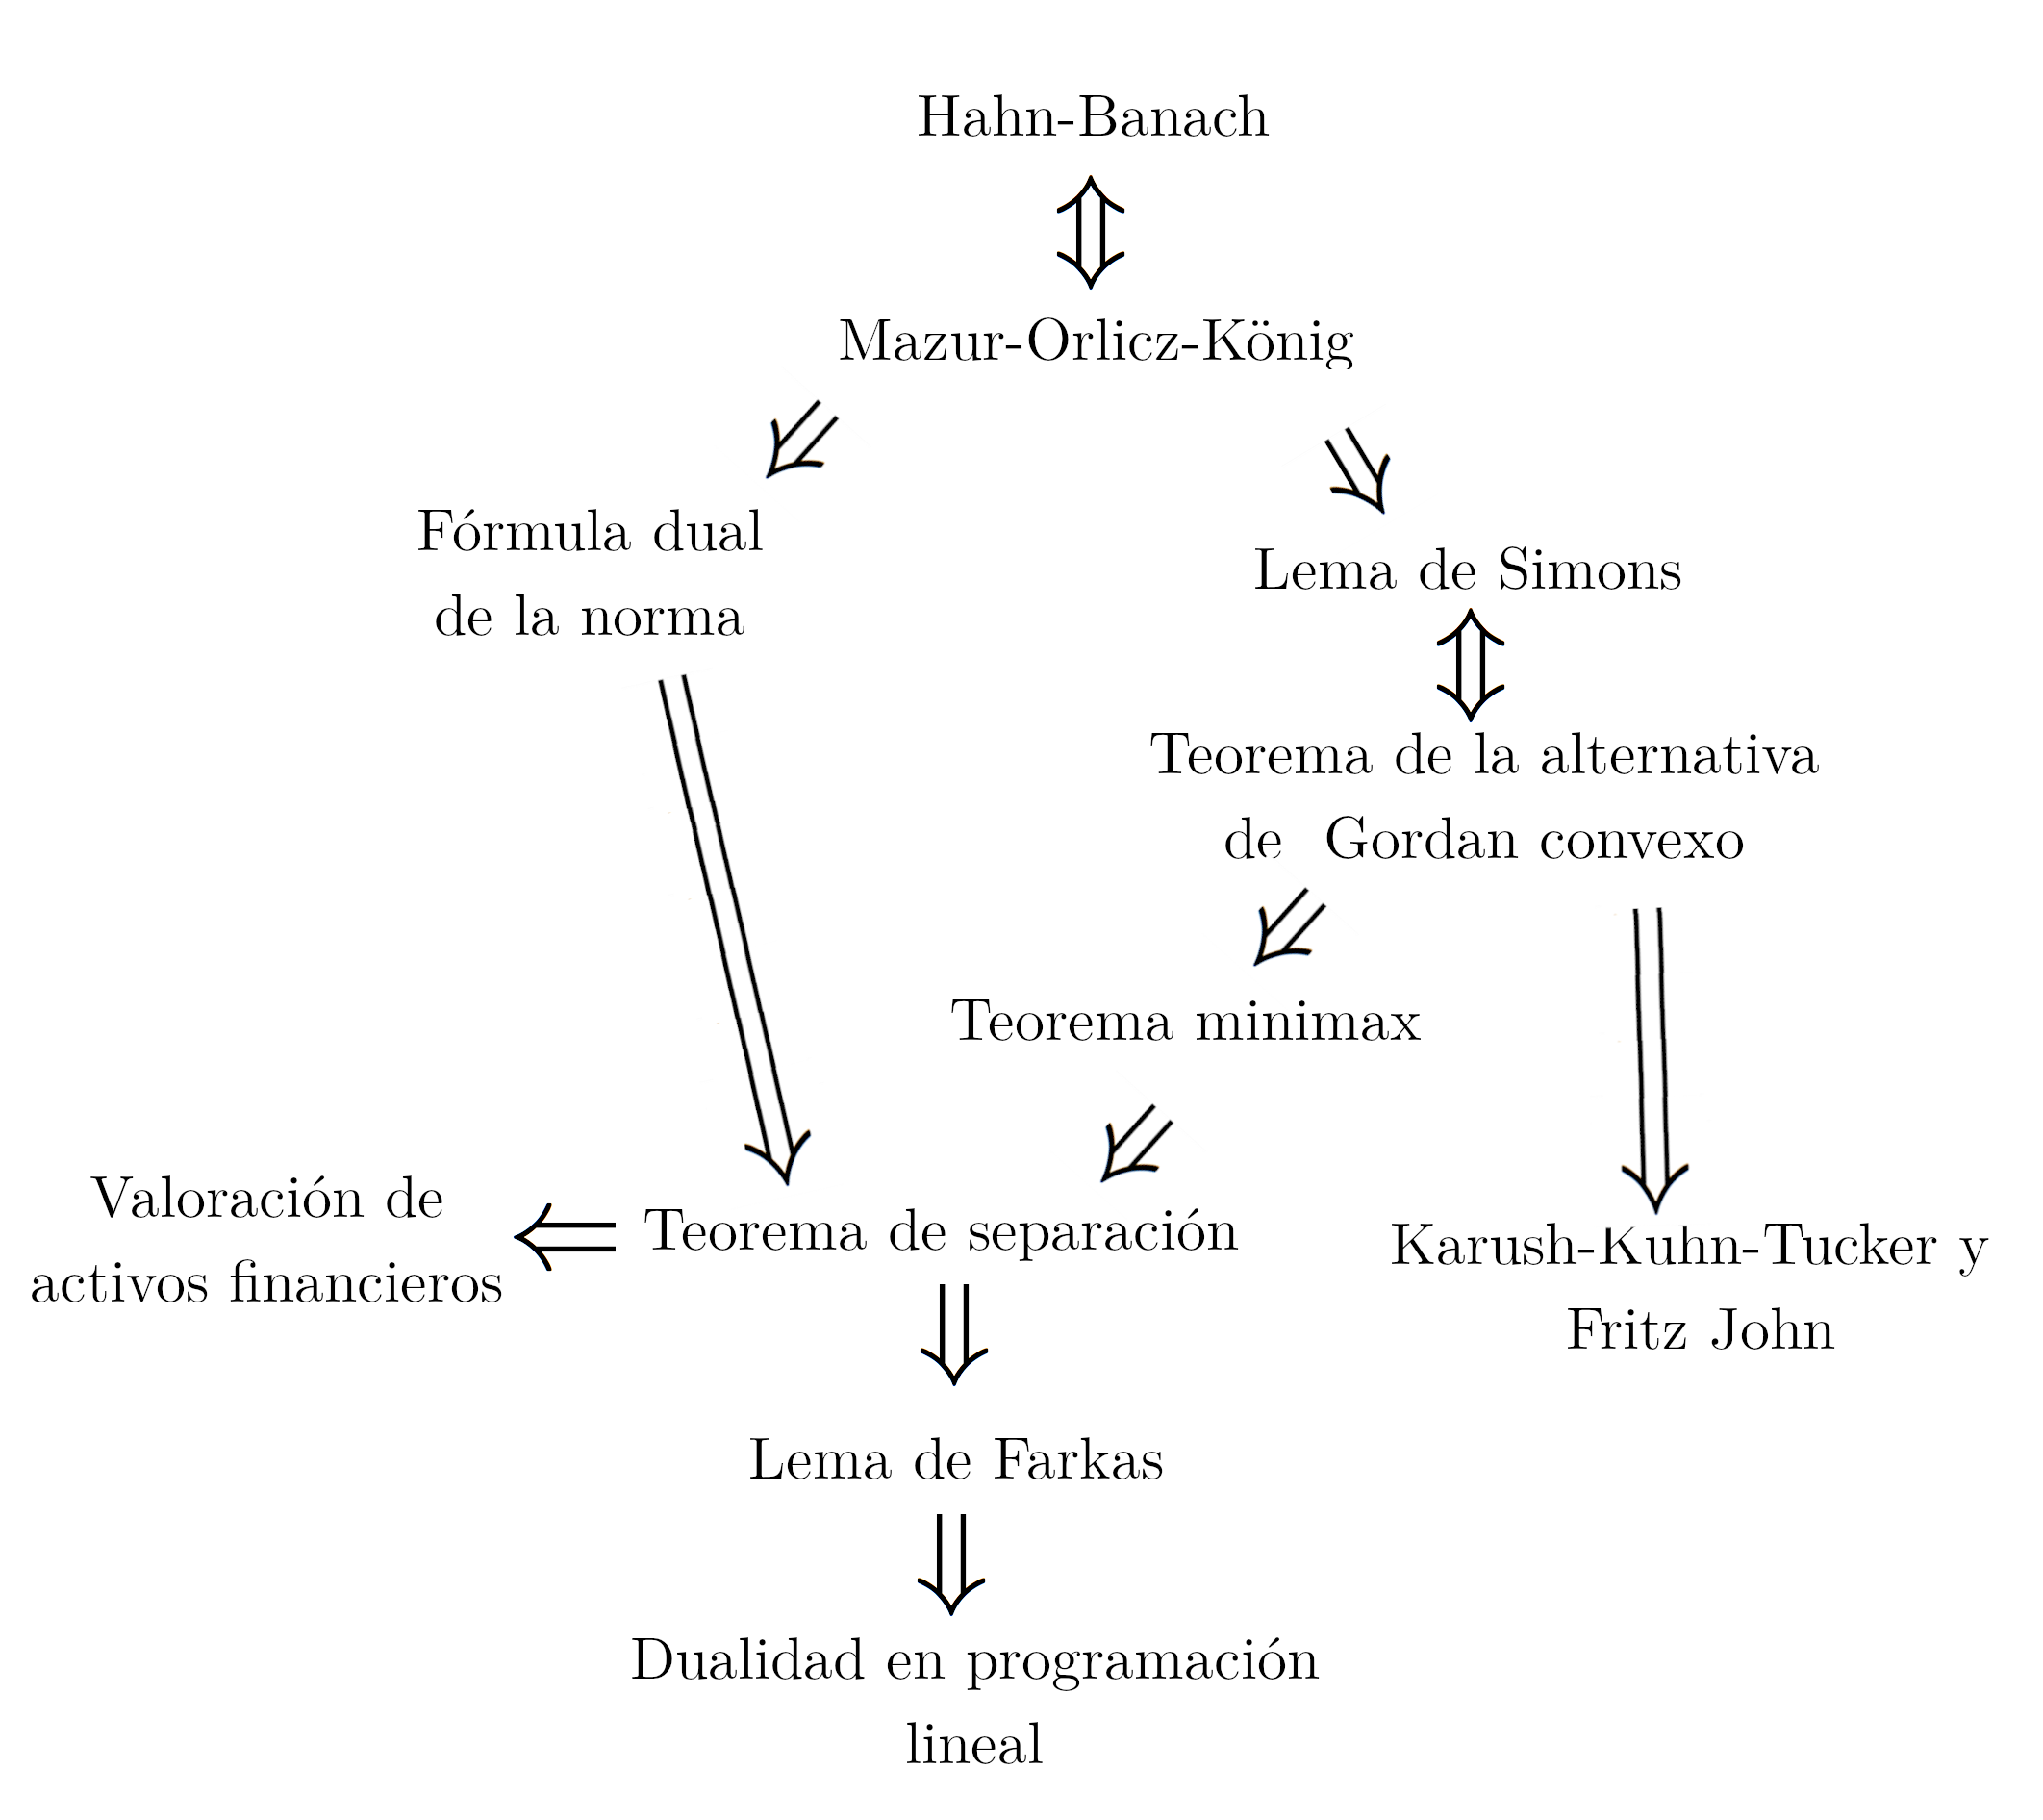
\includegraphics[width=0.9\linewidth]{imagenes/esquema.png}
	\label{fig:aux2}
\end{figure}

Como puede observarse, las técnicas son de carácter convexo y analítico funcional.

\section*{Informática}
Tras la concreción del tema a resolver dentro del ámbito del digitalizado 3D, se decidió empezar a trabajar en uno de los algoritmos más conocidos para ello, el \textit{Iterative Closest Point} (ICP). También, al comenzar el trabajo, se decidió la manera de realizar las pruebas necesarias. Se optó por la realización de un banco de pruebas utilizando \textit{OpenGL} (versión 4.6) como biblioteca gráfica, \textit{C++} como lenguaje de programación así como \textit{Qt} (versión 5.9.1) para la interfaz gráfica. El IDE, por lo tanto, ha sido \textit{Qt Creator 4.3.1} Este banco de pruebas debe proporcionar herramientas básicas para la manipulación de las nubes de puntos con las que estamos trabajando así como otras funcionalidades necesarias para el desarrollo de los distintos algoritmos. En este caso se hizo necesaria solventar problemas como: abrir y guardar archivos, manipulación de la matriz de vista, selección de un conjunto de puntos y borrado de los mismos, selección de puntos aislados, etc.\\

Volviendo al primer algoritmo a estudiar, se comprobó que era necesario un conocimiento previo acerca de los cuaternios, tanto para la demostración de la convergencia del método como para su implementación. Una vez completado, se procedió a la elaboración de distintas pruebas. Destacar que también se hizo necesario el cálculo de valores propios de una matriz por lo que se optó por usar al biblioteca \textit{Eigen} (en su versión 3.3.7). Posteriormente, se planteó la posibilidad de incluir mejoras al método usando la variación de las normales para obtener información acerca de la geometría del modelo. Por ello, fue necesaria la inclusión de esta opción dentro del banco de pruebas así como un algoritmo de simplificado de la nube de puntos tal y como se explicará en el desarrollo del trabajo. \\

Llegados a este punto, se planteó la posibilidad de incluir otra serie de mejoras al procedimiento o de estudiar otros algoritmos diferentes. Se siguió la segunda opción con el fin de tener una visión general más general del problema. Por ello, en último lugar a aparece un estudio acerca del algoritmo \textit{Random Sample Consensus} (RANSAC), partiendo de la explicación de los pasos del propio algoritmo pasando por razonamientos probabilísticos para asegurar la obtención de buenos resultados y finalmente la realización de pruebas del mismo.